\section{Conceptos básicos}

En la presente sección se pretende introducir los conceptos básicos de Inteligencia Artificial, Aprendizaje Automático (\textit{Machine Learning}), Aprendizaje Profundo (\textit{Deep Learning}) y Visión Computarizada (\textit{Computer Vision}) necesarios para comprender el presente trabajo.

\begin{figure}[h]
\centering
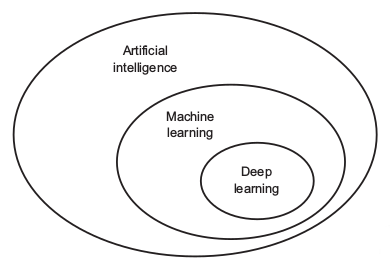
\includegraphics[width=0.5\textwidth]{imgs/marcoteorico.png}
\caption{Inteligencia Artificial, Aprendizaje Automático y Aprendizaje Profundo. \cite{Cho17}}
\end{figure}

\subsection{Inteligencia artificial}

En 1956, los padres de la \textit{Inteligencia Artificial}: Allen Newell, Herbert Simon, John McCarthy, Marvin Minsky y Arthur Samuel acuñaron el término \textit{``Inteligencia Artificial''} como \textit{``una rama de las Ciencias de la Computación que tiene como objetivo simular comportamiento inteligente en una computadora.''} \cite{ensayo-samuel} \cite{allen-newell}

En un principio dichos sistemas estaban dotados de una gran cantidad de reglas que los hacían muy efectivos para resolver ciertos problemas donde los pasos están bien definidos y son lógicos.

Entre las décadas del ’50 y ’80 se creyó que con un conjunto suficientemente grande de reglas se podría lograr una inteligencia al nivel de los humanos. 
No obstante ciertos problemas como el reconocimiento de objetos en imágenes o de transcripción de texto a partir de sonido son difíciles de tratar con este enfoque, a pesar de que los humanos lo pueden realizar sin dificultad. Y esencialmente la dificultad de estos problemas radica en que es complejo obtener un conjunto de reglas o pasos algorítmicos para resolverlos.

\subsection{ Aprendizaje automático } \label{aprendizaje-automatico}

En 1962 Arthur Samuel en su ensayo \textit{``Artificial Intelligence: A Frontier of Automation''} \cite{ensayo-samuel} propone construir algoritmos donde el flujo del programa dependa de ciertos pesos asignados por un mecanismo en función de la \textit{performance} calculada, de modo que las máquinas ``aprendan'' de su experiencia. 
Éste fue un puntapié inicial para la fundación del campo del \textit{aprendizaje automático}, el cual consiste en el estudio de algoritmos que mejoran automáticamente su rendimiento gracias a la experiencia.

\begin{figure}[h]
\centering
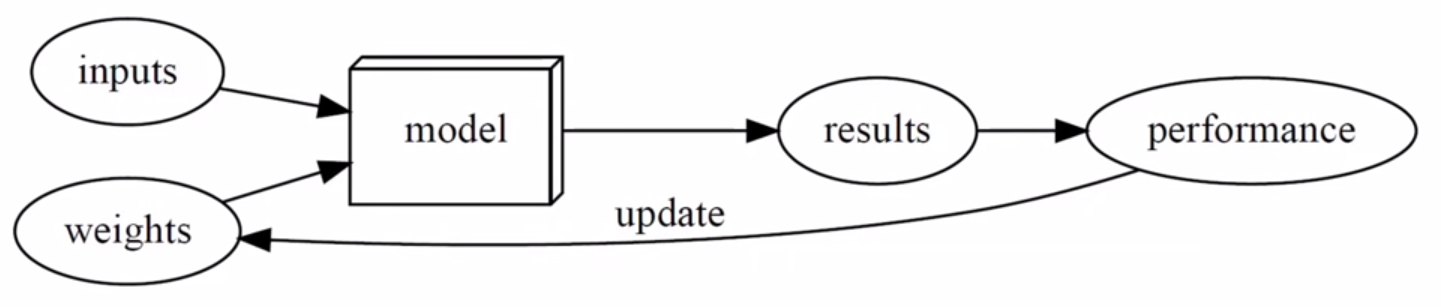
\includegraphics[width=1\textwidth]{imgs/automated-learning.png}
\caption{ Esquema de la estructura propuesta por Arthur Samuel. \cite{fastbook}}
\end{figure}

Tom Mitchell define en su célebre libro
 \textit{``Machine learning''} (1997, \cite{mitchell}) al aprendizaje automático como:

\begin{quote}
``Se dice que un programa de computadora aprende de la experiencia $E$ respecto a una tarea $T$ y una medida de desempeño $P$ , si el desempeño medido con $P$ en una tarea $T$ , mejora con la experiencia $E$.''
\end{quote}

De este modo los algoritmos de aprendizaje automático construyen un modelo con el objeto de realizar predicciones o tomar decisiones sin haber sido expresamente programados para hacerlo.
El modelo es construido en base a entradas suministradas. \\

La flexibilidad de las técnicas han ido aumentando y actualmente se pueden aplicar a gran variedad de problemas como reconocimiento de imágenes, sonidos, generación de texto, entre otros.
%\subsubsection{Clasificaciones dentro del Aprendizaje Automático}
\\
Dependiendo del tipo de experiencia suministrada se suele distinguir entre distintos problemas de aprendizaje \cite{rusell}:
\begin{itemize}
    \item \textbf{Supervisado:} se suministran los resultados esperados para las entradas ejemplo. El objetivo del modelo es ``aprender'' la relación entre las entradas y las salidas de modo que frente a nuevas entradas produzca razonables resultados. Es por ello que a menudo a estos últimos se los llamará también \textit{predicciones}.
    \item \textbf{No supervisado:} sólo hay entradas (no hay salidas) y el objetivo es entender la estructura fundamental de los datos y aprender relaciones ocultas importantes.
\end{itemize}

Dependiendo de las predicciones del modelo en el caso supervisado hablaremos de:
\begin{itemize}
    \item \textbf{Regresión:} si las predicciones son valores continuos.
    \item \textbf{Clasificación:} Si las predicciones pertenece a un dominio de valores discreto.
    A su vez hablaremos de \textit{clasificación binaria} si las predicciones poseen sólo dos valores posibles.
\end{itemize}

En el presente trabajo trataremos un problema de clasificación binaria mediante \textit{aprendizaje supervisado}.

\subsection{Terminología del Aprendizaje Automático}

En esta sección veremos con más formalidad los conceptos que atañen al \textit{Aprendizaje Automático}. Además introduciremos la jerga específica utilizada en el mismo. Una vez leídas todas las definiciones recomendamos volver a la sección \ref{aprendizaje-automatico} (\textit{``Aprendizaje Automático''}) para constatar que detrás de la rigurosidad de símbolos y terminología específica se esconde sencillamente el modelo imaginado por Arthur Samuel en 1962. \cite{ensayo-samuel} \\

Como se aclaró en la sección anterior, en el presente trabajo trabajaremos con un problema de aprendizaje supervisado. En dichos problemas tenemos un conjunto de ejemplos $D$ formado por entradas para las cuáles poseemos una (única) salida conocida. A este conjunto se lo denomina \textbf{conjunto de datos} (o \textbf{\textit{dataset}}):
\begin{equation*}
    D = \{ (x, y) \} \quad D \subset A \times B,
\end{equation*}
donde $x$ es un vector real de $p$ dimensiones ($x \in \mathbb{R}^p$) llamado \textbf{variable independiente} o  \textbf{vector  de características}. A cada componente del mismo se lo llama \textbf{característica} (o \textit{\textbf{feature}}).
%    $A$ será el subconjunto de posibles valores válidos de nuestra variable independiente: $A \subseteq \mathbb{R}^p$.
Por otro lado, $y$ es llamada \textbf{variable dependiente u objetivo} (o \textit{\textbf{target}}). En caso de tratarse de un problema de regresión $y$ es una variable continua ($B \subseteq \mathbb{R} $). Si tenemos un problema de clasificación se la llama también \textbf{etiqueta} (o \textit{\textbf{label}}). En este caso $B$ será el conjunto de clases posibles ($|B| \in \mathbb{N} $). Por ejemplo, $B = \{``gato'', ``perro''\}$ para un clasificador que distinga fotografías de gatos y perros. \\
    
    
Llamaremos $I$ al conjunto de todas las entradas y salidas posibles para nuestro problema. $I$ generalmente es infinito puesto que todas las posibles entradas $A$ suele ser infinito:

\begin{equation*}
    I = A \times B.
\end{equation*}

Volviendo al problema de clasificar imágenes de gatos y perros, $A$ sería el conjunto (infinito) de todas las posibles imágenes que sean razonables recibir para dicho clasificador (imágenes donde haya algo discernible como gato o perro). A su vez, $I$ será el conjunto de dichas imágenes junto su respectiva etiqueta.\\

Generalmente $D$ es finito ($|D| \in \mathbb{N} $) ya que son los datos que poseemos (para los cuales conocemos certeramente una relación entre una entrada y su esperada salida). En este caso el conjunto de entradas disponibles $D$ no es exhaustivo y existen muchas otras entradas factibles desconocidas que constituyen el \textbf{espacio problema}:
\begin{equation*}
    D \subset I.
\end{equation*}

En una aplicación real, los casos futuros a clasificar serán elementos de $I - D$.\\

El objetivo del problema es ``aprender'' una función $f : A \rightarrow B$ que le asigna a cada entrada una salida. El objetivo no es sólo que prediga bien $D$ sino que posea una buena \textbf{generalización} al espacio problema $I$.\\

Como el conjunto de datos no es exhaustivo ($I - D \neq \emptyset$). Y existen infinitas entradas que no aparecen en el conjunto de datos, luego existen infinitas $f$ consistentes con los datos (que los interpolan):
\begin{equation*}
    \mathbb{H} = \{ f~|~f(x)=y ~\forall (x,y) \in D \}
\end{equation*}
%Todo punto no perteneciente a $D_t$ tiene la misma probabilidad para cualquier valor de predicción posible:
%\begin{equation*}
    %P( \hat{f}(x)=y~|~D_t ) = P( \hat{f}(x)=y'~|~D_t ) ~ con ~ %x \notin D_t~ \forall y,y' \in B
%\end{equation*}
Es por ello que debemos descartar algunas hipótesis, para lo cual se hacen suposiciones de la solución. Esto constituye lo que se llama \textbf{sesgo inductivo} o \textbf{base inductiva}.  \\

Por ejemplo podemos hipotetizar que $f$ es una combinación lineal de las características:
\begin{equation*}
    f(x) = \sum_{i=1}^n c_i . x_i 
\end{equation*}

Nuestro \textbf{modelo} lo constituirán tanto dicha fórmula (producto de nuestras asunciones) como los valores de los coeficientes. 

Las predicciones del modelo dependerán de la elección de dichos coeficientes, también denominados \textbf{parámetros} o \textbf{pesos} (o \textbf{\textit{weights}}). Para encontrar valores adecuados para los parámetros se utiliza un \textbf{algoritmo de optimización}, teniendo en cuenta un subconjunto $D_t$ de los datos disponibles $D$ ($D_t \subset D$). Esto es lo que se conoce como \textbf{fase de aprendizaje}. Durante este proceso se habla de \textbf{ajuste de los datos de entrenamiento}, \textbf{ajuste de los pesos} o simplemente \textbf{ajuste del modelo}. A $D_t$ se lo llama \textbf{conjunto de entrenamiento}. A continuación veremos por qué es importante no utilizar la totalidad de los datos disponibles para ajustar los pesos. \\

También, deberá existir una manera de medir la performance del modelo a partir de los resultados del mismo y de entradas y salidas conocidas. A esto se lo denomina \textbf{métrica}: es una función de las \textbf{etiquetas} y \textbf{predicciones}.
\begin{equation*}
    metric( f(x), y )
\end{equation*}

El objetivo del modelo es tener una buena performance sobre todo el conjunto de entrada $I$. Como se dijo, en la práctica los casos de $I-D$ pueden ser casos futuros sobre los que se utiliza el modelo para tomar decisiones en función de las predicciones.

Es muy importante contar con ejemplos adicionales $D_v$ para los cuales se conozcan tanto entradas como salidas ($D_v \subset D$) y que no pertenezcan al conjunto que se utilizó para el ajuste del modelo ($D_t \cap D_v = \emptyset$). De modo que midiendo en $D_v$ la performance podamos cuantificar la \textbf{capacidad de generalización} del modelo, entendiéndose a esta como la capacidad de extrapolar los resultados de $metric$ a casos nos vistos durante el entrenamiento.

A dicho conjunto $D_v$ lo denominamos \textbf{conjunto de validación}. 
Si el conjunto de validación ha sido bien elegido (más adelante veremos que $D_t \cap D_v = \emptyset$ es condición necesaria pero no siempre suficiente) las métricas calculadas en dicho conjunto serán una buena estimación de las métricas esperadas en el resto de los casos no observados:
\begin{equation*}
    \mathbb{E}_{(x,y) \in D_v} [metric(f(x),y)]  \approx \mathbb{E}_{(x,y) \in E} [metric(f(x),y)]
\end{equation*}
Trasladado a un ejemplo práctico, esto quiere decir que nos dará una pauta confiable de la performance de nuestro modelo en la aplicación final. Es por ello que crear de forma correcta el conjunto de validación es crítico. La etapa de medir la performance del modelo sobre $D_v$ suele llamarse \textbf{fase de evaluación}.\\

Las elecciones que constituyen la base inductiva del modelo (elección del modelo, variables de configuración del mismo, estrategias de entrenamiento, etc) constituyen ``parámetros que actuarán sobre los parámetros del modelo''. Es por ello que estas elecciones son denominadas \textbf{hiperparámetros}. Éstos no son modificados (o \textit{ajustados}) por medio del mecanismo de optimización que actúa sobre los pesos, pero a menudo se prueban diferentes valores de hiperparámetros (entrenando diferentes modelos) y se elige el que tenga mayor performance en la fase de evaluación. Al usar el conjunto de validación de este modo el modelo finalmente elegido deja de ser independiente del conjunto de validación, por lo que se suele realizar una evaluación final sobre un tercer conjunto $D_h$ ($D_h \subset D$ y disjunto respecto $D_t$ y $D_v$) denominado \textbf{conjunto de test} para obtener la métrica de generalización del resultado final. \\

Es frecuente denominar \textbf{conjunto de desarrollo} a la unión del conjunto de entrenamiento y el conjunto de validación ($D_t \cup D_v$). El nombre proviene de que estos datos se utilizan durante el \textit{desarrollo} de la solución: el conjunto de entrenamiento para ajustar los parámetros del modelo y el conjunto de validación para elegir los hiperparámetros. El conjunto de test, en cambio, se reserva exclusivamente para la evaluación final y no debe influir en ninguna decisión de diseño.\\

Luego de evaluado un modelo, está en condiciones de utilizárselo en la aplicación final. La acción de aplicar el modelo a un ejemplo al cuál no se conoce su resultado suele denominarse \textbf{inferencia}.

\subsection{Dilema sesgo-varianza y sobreajuste}

Sea:
\begin{itemize}
    \item $Y$ la variable dependiente a predecir.
    \item $X$ los atributos (variable independiente) en los que se basa la predicción.
    \item $f$ la función a predecir (relación subyacente entre $X$ e $Y$).
    \item $\epsilon$ el ruido en los datos, distribuido normalmente con media $0$ y varianza $\sigma$
\end{itemize}
Tenemos la fórmula:
\begin{equation*}
    Y = f(X) + \epsilon
\end{equation*}
Sea $f$ el modelo que intenta aproximar $f$, el error cuadrático de predicción para un ejemplo $x$ resulta ser:
\begin{equation*}
    Error(x) = \mathbb{E}[(Y - f(x))^2]
\end{equation*}

En \cite{Hastie} se definen:
\begin{equation*}
    Sesgo = \mathbb{E}[f(x)] - y]
\end{equation*}
\begin{equation*}
    Varianza = \mathbb{E}[~(f(x) - \mathbb{E}[f(x)])^2~]
\end{equation*}
\begin{equation*}
    ErrorIrreducible = \sigma
\end{equation*}

Reescribiendo la fórmula del error como:
\begin{equation*}
    Error(x) = Sesgo^2 + Varianza + ErrorIrreducible
\end{equation*}
En donde cada término del error puede ser interpretados como causas diferentes del mismo. 

Haciendo un análisis de la composición del error, interpretando cada causa:
\begin{itemize}
    \item \textbf{Error irreducible}: producto de la varianza en la función que se quiere predecir, ruido en los datos, etc. Está fuera de nuestro control.
    \item \textbf{Sesgo}: diferencia entre la predicción promedio de nuestro modelo, y el valor correcto que intentamos predecir. Puede ser pensado como el error causado por asunciones simplistas del modelo, como por ejemplo tomar que la distribución de los datos es lineal.
    \item \textbf{Varianza}: es la variabilidad de la predicción de un modelo, es decir, cuánto varía $f(x)$ alrededor de su media. Modelos con alta varianza ``prestan mucha atención'' a los datos de entrenamiento, corriendo el riesgo de no generalizar tan bien en datos no incluidos en el entrenamiento.
\end{itemize}

Cuando ajustamos los datos de entrenamiento con mayor precisión correemos el riesgo de que el modelo se adapte demasiado a los datos de entrenamiento, y no generalice bien en los datos de validación. Este escenario es denominado \textbf{sobreajuste} (o \textit{\textbf{overfitting}}). Cuando esto ocurra, las métricas mostrarán mucho peores resultados en el conjunto de validación que en el de entrenamiento.

En contraste si no se ajusta lo suficiente a los datos de entrenamiento poseerá un alto sesgo. Esto es lo que se conoce como \textbf{subajuste} (o \textit{\textbf{underfitting}}). A diferencia del sobreajuste, en este caso el error se manifestará tanto en la validación como en el entrenamiento.

\begin{figure}[H]
\centering
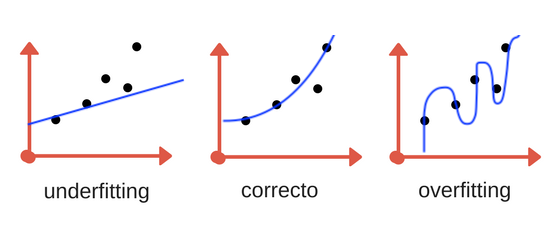
\includegraphics[width=0.85\textwidth]{imgs/overfitting.png}
\caption{ La imagen esquematiza que la elección de una base inductiva demasiado simple y poco expresiva puede ser el origen de un sesgo alto.
A su vez, modelos complejos que se pueden ajustar demasiado a los datos de entrenamiento pueden generar sobreajuste.}
\end{figure}

Es por ello que los modelos más complejos, al tener más capacidad expresiva, pueden ajustar mejor los datos de entrenamiento (y potencialmente sobreajustar). El error de entrenamiento tiende a decrecer cuando incrementamos la complejidad del modelo.

\begin{figure}[H]
\centering
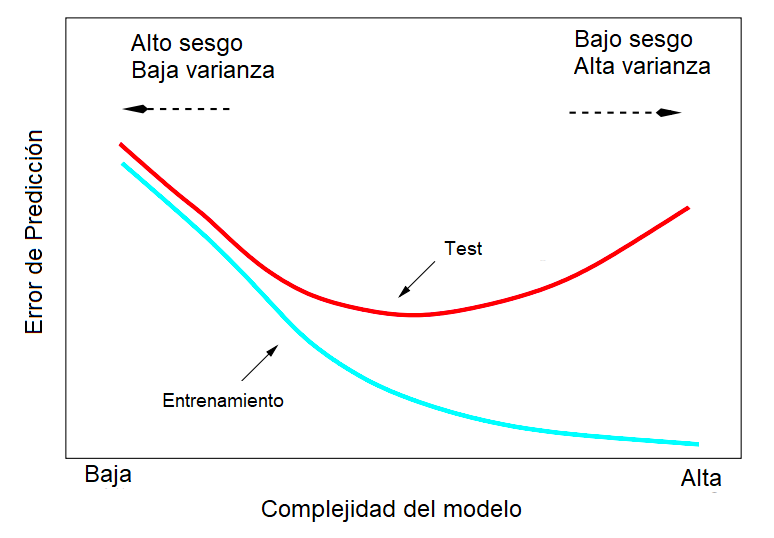
\includegraphics[width=0.95\textwidth]{imgs/complejidad-error.png}
\caption{ La gráfica esquematiza que cuando la complejidad de nuestro modelo crece, la varianza tiende a aumentar en tanto que el sesgo disminuye. Lo opuesto sucede cuando la complejidad del modelo disminuye. \cite{Hastie}}
\end{figure}

Esto último no quiere decir que siempre la primer solución al sobreajuste sea reducir la complejidad del modelo. Como dijimos, esta última aumenta la capacidad expresiva y por ende la \textit{capacidad} de sobreajustar. No obstante en métodos de optimización iterativos (como el empleado con las redes neuronales) podemos controlar la cantidad de ajuste por medio del número de iteraciones. Ya veremos que existen formas de combatir el sobreajuste y entrenar modelos más robustos llamados \textit{técnicas de regularización}.

Más adelante veremos que reducir la complejidad de los modelos ante la presencia del sobreajuste no es -generalmente- la mejor opción en el caso del Aprendizaje Profundo. De hecho, la práctica demuestra que es la última de las opciones a intentar entre un gran abanico de soluciones. Como veremos en la subsección \ref{subsection:representaciones}, en el aprendizaje profundo la gran complejidad de los modelos es lo que permite aproximar funciones complejas que reciban los \textit{``datos crudos''} (por ejemplo valores de píxeles en caso de imágenes) y calculen las representaciones idóneas para el proceso de clasificación. Esto constituye el gran éxito del aprendizaje profundo por sobre anteriores enfoques que consistían en extraer características con algún algoritmo \textit{ad-hoc} específico al dominio y tan solo luego utilizar un clasificador de aprendizaje automático.

El sobreajuste afecta a la mayoría de los métodos de Aprendizaje Automático. Es importante por ello contar con un conjunto de validación para medir las métricas elegidas en datos que no se usaron para entrenar.

\subsection{Conjunto de validación}

Como se dijo en secciones anteriores, se utiliza un \textbf{conjunto de datos de validación} $D_v$ no incluídos en el entrenamiento para medir la capacidad de generalización del modelo. 

Ya que nuestro objetivo final es aplicar el modelo en datos nunca antes vistos, $D_v$ debe ser representativo del conjunto de entradas factibles $E$.

De manera obvia, los datos de validación deben no aparecer entre los datos de entrenamiento $D_t$:
\begin{equation*}
    D_v \cap D_t = \emptyset
\end{equation*}
A menudo se toma una partición aleatoria de los datos. Pero también debe evitarse cualquier correlación con los datos de entrenamiento $D_t$ que no sea extensible al conjunto de entradas factibles $E$.

 Un ejemplo dónde, claramente, no es válido partir aleatoriamente las entradas para construir los conjuntos de entrenamiento y validación es las series temporales (véase figura \ref{fig:validacion-ts}). De hacerlo es fácil para el modelo aprender valores certeros teniendo valores conocidos durante el entrenamiento dentro del entorno cercano del valor a predecir. Contrariamente a este escenario, en una aplicación real probablemente querramos predecir valores \textit{futuros}. Por lo que una correcta partición tomaría un rango continuo de los últimos valores para confeccionar un conjunto de validación representativo.\\

Al ser un punto tan crítico la creación de un buen conjunto de validación suele ser fuente de numerosos errores en aplicaciones prácticas.

\begin{figure}[H]
\begin{subfigure}{0.33\textwidth}
\centering 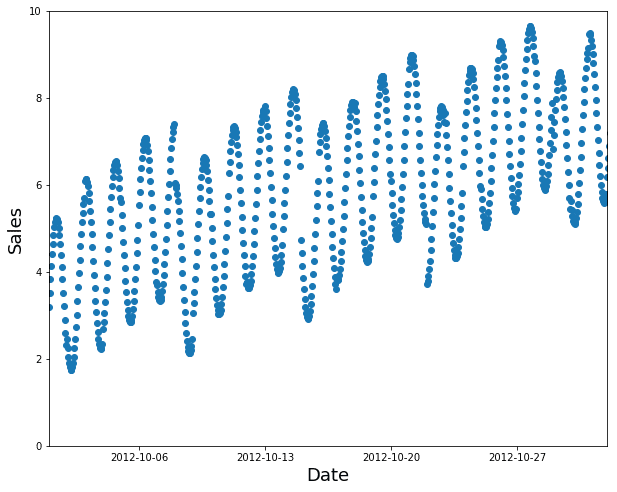
\includegraphics[width=0.3\textwidth]{imgs/ts11.png}
\end{subfigure}
\begin{subfigure}{0.33\textwidth}
\centering 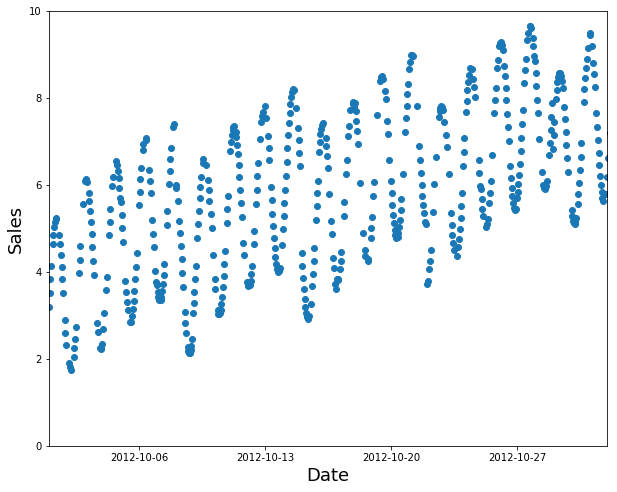
\includegraphics[width=0.3\textwidth]{imgs/ts2.png}
\end{subfigure}
\begin{subfigure}{0.33\textwidth}
\centering 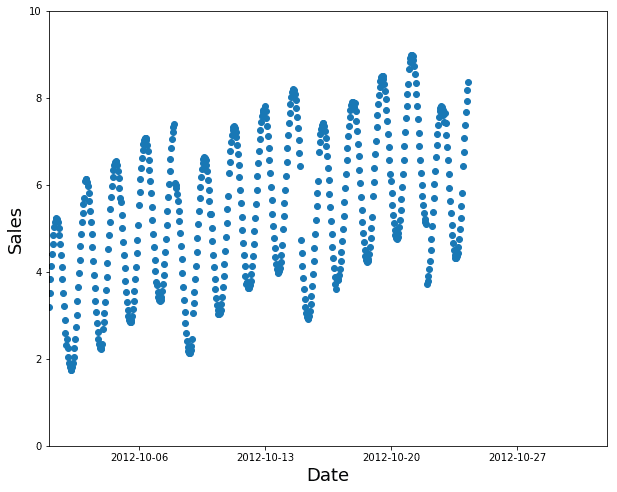
\includegraphics[width=0.3\textwidth]{imgs/ts3.png}
\end{subfigure}
\caption{ La primer figura muestra una serie temporal. La segunda muestra un subconjunto aleatoriamente seleccionado de ejemplos. La última muesta un subconjunto de entrenamiento correctamente seleccionado: siendo la validación un rango continuo de los últimos valores.  Fuente: \cite{fastai-validation} }
\label{fig:validacion-ts}
\end{figure}

En conjuntos de datos académicos es frecuente que la separación en conjunto de validación ya esté dada con el mismo conjunto para que los resultados de diversas investigaciones sean comparables de forma correcta.\\


\subsubsection{Validación cruzada}

El método de validación cruzada (descripto en \cite{berrar}) consiste en entrenar y evaluar modelos sobre diferentes particiones de entrenamiento y validación y combinar los resultados de los valores de las métricas obtenidos (por ejemplo tomando el promedio).

Existen diferentes estrategias de validación cruzada:
\begin{itemize}
    \item \textbf{K-iteraciones} (o \textit{K-folding}): consiste en particionar los datos disponibles en $k$ grupos y hacer $k$ iteraciones. En la $i$-ésima se utiliza el grupo $i$ para validación y el resto se lo usa para entrenamiento.
    \item \textbf{Aleatoria}: consiste en hacer $k$ iteraciones donde se elijen aleatoriamente la partición de validación. Como ventaja el tamaño de la partición no depende del número de iteraciones. Dentro de las desventajas destaca que existe la probabilidad de que existan ejemplos que no sean incluídos en ninguna validación.
    \item \textbf{Dejando uno afuera}: consiste en hacer $N$ iteraciones (siendo $N$ la cantidad de muestras disponibles). En la $i$-ésima iteración se utilizan todos los datos para entranar excepto el $i$-ésimo elemento del conjunto que se usa para evaluación.
\end{itemize}

\begin{figure}[h]
\centering
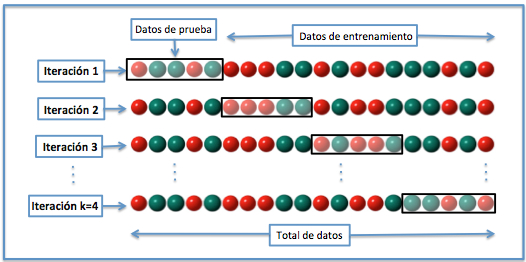
\includegraphics[width=1\textwidth]{imgs/Kfold_cross_validation.jpg}
\caption{Método de validación cruzada de K-iteraciones. Fuente: \cite{image-cross-validation}}
\end{figure}

La limitación de la validación cruzada es el gran esfuerzo computacional. Esto es debido a que se deben ejecutar $k$ entrenamientos independientes. 

Por lo que se utiliza validación cruzada mayormente cuando se cuenta con pocos datos. Es muy útil, también, en casos donde el puntaje de validación suele no ser preciso debido a que varía demasiado al cambiar la partición de validación elegida (generalmente sucede cuando se posee pocos datos y el conjunto de validación es demasiado pequeño). Así, eligiendo diferentes particiones y promediando el puntaje, se obtiene un estimador de menor varianza del puntaje real o de generalización.

Un dato importante a tener en cuenta es que muchos esquemas de validación cruzada son sólo aplicable cuando uno puede particionar aleatoriamente los datos para obtener un conjunto de validación representativo.


\subsection{Elección de hiperparámetros}

Como se mencionó en anterioremente, generalmente se exploran diferentes elecciones de hiperparámetros. A este procedmiento a veces se lo conoce como \textbf{puesta a punto del modelo} o \textit{\textbf{model tunning}} (no confundir con \textit{fine tunning} que es la técnica de re-utilizar un modelo ya entrenado en otros conjuntos de datos, explicado más adelante en el trabajo).

Existen diferentes estrategias para la exploración de hiperparámetros tales como:
\begin{itemize}
    \item \textit{\textbf{Grid Search:}} se prueban todas las asignaciones posibles para conjuntos de valores propuestos para cada hiperparámetro.
    \item \textit{\textbf{Random Search:}} se prueban asignaciones aleatorias de los hiperparámetros dentro de un conjunto de valores propuestos para cada uno.
    \item \textbf{Optimización Bayesiana:} utiliza el método bayesiano de optimización global para maximizar funciones (para una descripción detallada ver \cite{bayesian}). Suele obtener mejores resultados que el \textit{Random Search} y requerir menor cómputo que \textit{Grid Search} por su capacidad de razonar acerca de las asignaciones que no han sido probadas, y así elegir cuáles probar.
    \item \textbf{Algoritmos genéticos:} parten de un conjunto de asignación inicial y genera otras cambiando aletoriamente algunos valores de hiperparámetros. Luego de cada paso se queda con las mejores asignaciones (de mayor performance).
    \item \textbf{Manualmente:} En la práctica suele ser poco factible entrenar el modelo varias veces para demasiadas asignaciones de hiperparámetros. Esto es especialmente cierto en el \textit{aprendizaje prufundo} donde el tiempo de entrenamiento es considerable.
    Comúnmente se prueban manualmente hiperparámetros que son conocidos en la literatura que funcionan bien por defecto. 
\end{itemize}

En general métodos exhaustivos como \textit{Grid Search} no se utilizan en la práctica por la demanda de tiempo que conlleva. Se suele ver en la literatura científica y sólo tienen sentido si se desea arribar a conclusiones sobre determinados hiperparámetros (también es visto su uso en \textit{competencias de modelos} donde diferencias mínimas en la performance permiten escalar en la tabla de posiciones).

Frecuentemente también se utilizan métricas y visualizaciones para analizar la estabilidad del entrenamiento, convergencia del proceso de optimización y otras heurísticas, por medio de las cuales podemos estimar si es necesario variar determinado hiperparámetro. 

En el Capítulo 6 de FastBook \cite{fastbook}, por ejemplo, se explica cómo elegir el umbral de aceptación para un problema de clasificación multicategoría dónde la salida del modelo son probabilidades. Para ello se visualiza cómo varía la tasa de aciertos (calculada en el conjunto de validación) para diferentes valores del umbral (ver figura \ref{fig:umbralacc}).
Ahí mismo se explica que, como \textit{''regla heurística''} general, cuándo se eligen hiperparámetros de este modo raramente se estará sobreajustando el conjunto de validación si la gráfica de la métrica en función del hiperparámetros es suave.\\

\begin{figure}[h]
\centering
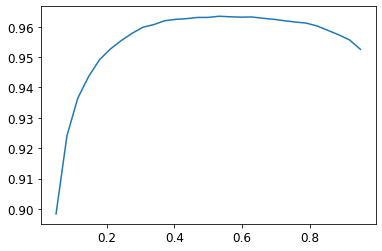
\includegraphics[width=0.8\textwidth]{imgs/accuracy_umbral.png}
\caption{ Tasa de aciertos en función al umbral de aceptación elegido para un problema de clasificación multi-categoría. Fuente: \cite{fastbook}.  }
\label{fig:umbralacc}
\end{figure}

Veremos más adelante en el presente trabajo algunas técnicas populares en la práctica del aprendizaje profundo que se utilizan a menudo para elegir manualmente hiperparémetros, incluso en circunstancias como competencias de modelos dónde hilar fino en las métricas es muy importante.
    

\subsection{Conjunto de test}

Las diferentes asignaciones de hiperparámetros son comparadas teniendo en cuenta las métricas sobre el conjunto de validación. Si se realizan demasiadas pruebas se corre el riesgo de ``sobreajustar los hiperparámetros'' y  que la performance que guia la elección de los mismos no generalice bien a conjuntos de datos no observados.\\

Como se explicó en secciones anteriores, se suele contar con un tercer conjunto de datos (además del de entrenamiento y de validación) denominado \textbf{conjunto de test}. El mismo se utiliza para realizar una evaluación final no sesgada del modelo. Ésto puede parecer un despropósito pero es necesario para seguir una metodología correcta y mantenernos intelectualmente honestos.\\

\subsection{Métricas} \label{ref:metrics}

Ya hemos introducido el concepto de \textbf{métricas} en las secciones anteriores donde explicamos que son funciones para medir la performance del modelo.

Las \textbf{metricas} (pueden considerarse varias) son problema-dependientes debido a que dependen tanto de la naturaleza de las predicciones y de las entradas como del objetivo para el cuál se utilizará el modelo. 

Deben poseer un significado interpertable por los usuarios en términos del uso que se le está dando al modelo.

No se debe confundir métrica con la \textit{función de costo} que utiliza el mecanismo automático de optimización del modelo y a menudo posee propiedades matemáticas deseables por el mismo. El concepto se tratará más detalladamente cuando se hable de descenso por gradiente en redes neuronales  (subsección \ref{subsection:descenso-gradiente}).

\subsubsection{Métricas en problemas de regresión}
En problemas de regresión podemos encontrar las métricas:
\begin{itemize}
    \item \textbf{Error cuadrático médio (MSE):} es una de las métricas más utilizadas en problemas de regresión puesto a qué es una función diferenciable. Pero penaliza los errores grandes, siendo suceptible a valores atípicos.
    \begin{equation*}
        MSE = \frac{1}{n} \sum_{i=1}^n ( y_i - \hat{f}(x_i) )^2
    \end{equation*}
    \item \textbf{Error absoluto médio (MAE): } no penaliza tanto a los errores grandes como MSE.
    \begin{equation*}
        MAE = \frac{1}{n} \sum_{i=1}^n | y_i - \hat{f}(x_i) | 
    \end{equation*}
    \item \textbf{Coeficiente de determinación ($R^2$)}: representa que proporción de la varianza de la variable dependiente $y$ es explicada por las características de la variable independiente $x$.
    \begin{equation*}
        R^2 = 1 - \frac{\sum_{i=1}^n ( y_i - \hat{f}(x_i) )^2}{\sum_{i=1}^n ( y_i - \overline{y} )^2} 
    \end{equation*}
    También puede ser pensada como una comparación del MSE de nuestro modelo con el del \textit{baseline} trivial de predecir la media de las entradas.
\end{itemize}

\subsubsection{Métricas en problemas de clasificación}
En problemas de clasificación podemos encontrar las métricas:
\begin{itemize}
    \item \textit{\textbf{Accuracy}} es una de las métricas más utilizadas en problemas de clasificación. Consiste simplemente en la proporción de aciertos realizados. También se la conoce como \textbf{tasa de aciertos}.
    \begin{equation*}
        Accuracy = \frac{1}{n} \sum_{i=1}^n Igual( y_i, \hat{f}(x_i) )
    \end{equation*}
    \begin{equation*}
        Igual(a,b) = \left\lbrace\begin{array}{c} 1~si~a = b \\  0~si~a \neq b \end{array}\right.
    \end{equation*}
    \item \textit{\textbf{Top k - Accuracy:}} para problemas donde el número de clases es grande y existen varias fácilmente confundibles entre sí usualmente se modifica el problema de clasificación permitiendo a la predicción ser un conjunto de $k$ elementos (para cierto $k$ fijo) y se mide como acierto si la clase objetivo pertenece a este conjunto de predicciones.
    \begin{equation*}
        Top~k-Accuracy = \frac{1}{n} \sum_{i=1}^n Acierto( y_i, \hat{f}(x_i) )
    \end{equation*}
    \begin{equation*}
        Acierto(etiqueta, predicciones) = \left\lbrace\begin{array}{c} 1~si~etiqueta \in predicciones \\  0~si~etiqueta \notin predicciones \end{array}\right.
    \end{equation*}
    \item \textbf{Matriz de confusión:} a menudo resulta útil calcular una matriz donde los ejes sean las etiquetas y las predicciones. De modo de contener en la casilla $M_{i,j}$ cuántos ejemplos de la clase $i$ han arrojado como resultado una predicción para la clase $j$.
    Los elementos de la diagonal representan los aciertos, mientras que los otros muestran errores.
    Es utilizada también debido a que confundir una clase por otra puede tener diferentes consecuencias prácticas y por lo tanto se puede preferir cierto tipo de errores a otros. Para comparar dos resultados y determinar cuál es mejor se pueden utilizar matrices de ponderación que le asignen a cada $M_{i,j}$ un costo $C_{i,j}$ ($C_{i,i} = 0$) de modo que el error quede definido como:
    \begin{equation*}
        Error = \sum_{i}\sum_{j}M_{i,j} \times C_{i,j}
    \end{equation*}
    De modo que $C_{i,j}$ refleje el costo práctico de cada tipo de error.
\end{itemize}

\begin{figure}[h]
\centering
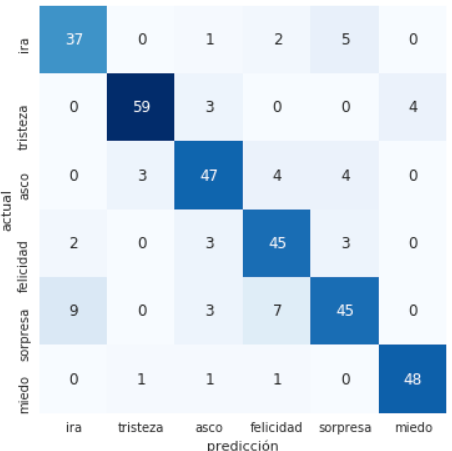
\includegraphics[width=0.45\textwidth]{imgs/confusion-matrix.png}
\caption{Ejemplo de una matriz de confusión para un problema de detección de emociones de 6 clases.}
\end{figure}

Dependiendo de la aplicación podemos querer optimizar diferentes métricas (y a menudo hay un \textit{trade-off} entre ellas). Por ejemplo en un problema de clasificación binaria para detectar tumores querremos que no se le pase ningún tumor maligno como beningno, a costa de arrojar un número razonable de falsas alarmas.\\

Es importante \textbf{siempre calcular las métricas en el conjunto de validación}. Las métricas sobre el conjunto de entrenamiento tienen poco sentido, se monitorean con la única utilidad de detectar cuándo el modelo está sobreajustando.

\subsubsection{Métricas en problemas de clasificación binaria}
\label{subsubsection:metricbinary}

Como ya comentamos, en el presente trabajo trataremos un problema de clasificación binaria. Es por ello que haremos especial énfasis en las métricas que atañan a ésta subcategoría de problemas de clasificación. 

En esta subcategoría de problemas suele denominarse a las clases como \textbf{positiva} y \textbf{negativa} \cite{metricas-binarias}. La decisión de a cuál clase definir como positiva y a cuál definir como negativa a veces es clara como por ejemplo en problemas de detección: la clase positiva será la etiqueta \textit{detectado} y la negativa \textit{no detectado}.

En nuestro caso querremos detectar errores en la confección de telegramas, buscando detectar \textit{no coincidencias} de firmas. Por eso trataremos como positiva a las \textit{no coincidencias}, ya que son las clases que se utilizará para desencadenar alertas en el sistema al cuál se pretende integrar la detección. En otros casos como en el problema de \textit{``Verificación Automática de Firmas Manuscritas''} \cite{tesis-parodi} se pretende verificar que la autoría de cierta firma es la que declara ser, comparándola con las de un autor registrado al que se le conocen ciertas firmas auténticas. En dicho trabajo se trabaja como clase positiva a la verificación de una firma como auténtica, o sea cuando coincide con las registradas del autor que declara ser. Es importante tener esto en cuenta a la hora de comparar métricas entre diferentes trabajos e implementaciones. \\

Luego de definidas las clases como positivas y negativas las predicciones del modelo pueden clasificarse en cuatro categorías en relación a su valor y al de la etiqueta respectiva según:

\begin{table}[h!]
\begin{tabular}{l|c|c|l}
\cline{2-3}
\textbf{}                                        & \multicolumn{1}{l|}{\textbf{Predicción Positiva}}                 & \multicolumn{1}{l|}{\textbf{Predicción Negativa}}                 &  \\ \cline{1-3}
\multicolumn{1}{|l|}{\textbf{Etiqueta Positiva}} & \begin{tabular}[c]{@{}c@{}}$TP$\\ (Verdadero Positivo)\end{tabular} & \begin{tabular}[c]{@{}c@{}}$FN$\\ (Falso Negativo)\end{tabular}     &  \\ \cline{1-3}
\multicolumn{1}{|l|}{\textbf{Etiqueta Negativa}} & \begin{tabular}[c]{@{}c@{}}$FP$\\ (Falso Positivo)\end{tabular}     & \begin{tabular}[c]{@{}c@{}}$TN$\\ (Verdadero Negativo)\end{tabular} &  \\ \cline{1-3}
\end{tabular}

\caption{Las abreviaciones TP, TN, FP, FN son populares en la literatura y provienen de los nombres en inglés, respectivamente: \textit{True Positive}, \textit{True Negative}, \textit{False Positive} y \textit{False Negative} }
\end{table}

Definirimos también (para simplificar la notación en las fórmulas) las super-categorías (constituída por uniones de las cateogrías definidas):
\begin{itemize}
    \item \textbf{Etiqueta Positiva}: conjunto de los datos que pertenecen a la clase positiva.
    \begin{equation*}
        P = TP+FN
    \end{equation*}
    
    \item \textbf{Etiqueta Negativa}: conjunto de los datos que pertenecen a la clase negativa.
    \begin{equation*}
        N = TN + FP
    \end{equation*}
    
    \item \textbf{Totalidad de datos}: conjunto de todos los datos usados para la evaluación.
    \begin{equation*}
        Total = FP+FN+TP+TN
    \end{equation*}
\end{itemize}

Luego se definen en función de las cardinalidades de dichas categorías diversas métricas para el problema de clasificación binaria (veáse \cite{metricas-binarias}), cada una con implicancias y significados distintos:
\begin{itemize}
    \item \textbf{Tasa de aciertos} (o \textit{\textbf{accuracy}}): simplemente la proporción de ejemplos clasificados correctamente.
    \begin{equation*}
        Accuracy = \frac{TP+TN}{Total}
    \end{equation*}
    
    \item \textbf{Ratio de error} (o \textit{\textbf{error rate}}): es el concepto complementario al de tasa de aciertos, la proporción de errores cometidos.
    \begin{equation*}
        Error~Rate = \frac{FP+FN}{Total} = 1 - Accuracy
    \end{equation*}
    
    
    \item \textbf{Exhaustividad} (\textit{\textbf{recall}} o \textbf{TPR} \textit{True Positive Rate}): la proporción de ejemplo positivos detectados como tales.
    \begin{equation*}
    Recall = \frac{TP}{TP+FN} = \frac{TP}{P}
    \end{equation*}
    En términos de probabilidad puede ser interpretado como la probabilidad de que nuestro modelo detecte un caso positivo.
    
    \item \textbf{Ratio de falsos negativos} (o \textbf{FNR} \textit{False Negative Rate}): es el concepto complementario a \textit{recall}:
    \begin{equation*}
    FNR = \frac{FN}{TP+FN} = \frac{FN}{P} = Miss~Rate = 1 - Recall
    \end{equation*}
    Puede ser interpretado como la probabilidad de que el modelo falle al detectar casos positivos. Por ello también se lo llama \textit{Miss Rate}.
    
    
    \item \textbf{Especificidad} (\textbf{\textit{Specificity}} o \textbf{TNR} \textit{True Negative Rate}): la proporción de ejemplo negativos detectados como tales.
    \begin{equation*}
    Specificity = \frac{TN}{FP+TN} = \frac{TN}{N}
    \end{equation*}
    En términos de probabilidad puede ser interpretado como la probabilidad de que nuestro modelo detecte un caso negativo.
    
    \item \textbf{Ratio de falsos positivos} (o \textbf{FPR} \textit{False Positive Rate}): es el concepto complementario a \textit{especificidad}:
    \begin{equation*}
    FPR = \frac{FP}{FP+TN} = \frac{FP}{N} = False~Alerts = 1 - Specificity
    \end{equation*}
    Puede ser interpretado como la probabilidad de que el modelo falle al detectar casos negativos. Por ello también se lo llama \textit{Falsas Detecciones} o \textit{Falsas Alertas}.
    
    
    \item \textbf{Precisión} (\textit{precision} en inglés): es la proporción de detecciones (predicciones positivas) que son correctas.
    \begin{equation*}
    \text{Precisión} = \frac{TP}{TP+FP} = \frac{TP}{\text{Predicción~Positiva}}
    \end{equation*}
    Puede interpretarse como qué tan probable es que una alerta por clase positiva esté bien, por eso también se lo denomina \textbf{poder predictivo positivo}.
\end{itemize}

\subsubsection{Métricas en el problema de Verificación Automática de Firmas Manuscritas} \label{subsubsection:metricasfirmas}

En aplicaciones reales es importante conocer las implicancias prácticas de las métricas y definir objetivos razonables (no se suele desarrollar sin un objetivo ya que no se sabría cuándo considerar que el trabajo es suficientemente bueno). Los objetivos deben proveer garantías prácticas a los usuarios y dependerán del uso de la aplicación. Por ello, siempre hay que tener presente para qué se usará el modelo que pretendemos crear a la hora de elegir la métrica y qué significado nos provee dicha métrica. \\

En la bibliografía de \textit{``Verificación Automática de Firmas Manuscritas''} \cite{tesis-parodi} se trabaja con las métricas:
\begin{itemize}
    \item \textbf{Tasa de Falsos Rechazos (FRR)}: porcentaje o ratio de rechazos de firmas auténticas.
    \item \textbf{Tasa de Falsa Aceptación (FAR)}: porcentaje o ratio de aceptaciones de falsificaciones.
\end{itemize}

El punto donde son iguales se suele llamar Tasa de error de intersección o \textbf{\textit{Equal Error Rate} (EER)}. De tratarse de un dataset con clases balanceadas será igual a la tasa de aciertos (ver figura \ref{fig:err}). \\

\begin{figure}[h]
\centering
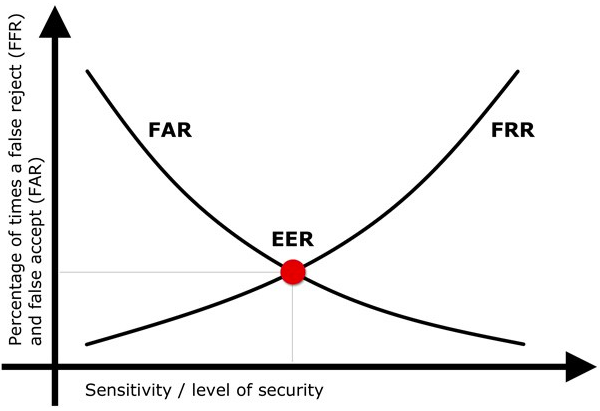
\includegraphics[width=0.5\textwidth]{imgs/err.png}
\caption{ La tasa de error de intersección es la elección del umbral de sensibilidad que representa un balance equitativo entre falsos positivos y falsos negativos. Créditos de la imagen: \href{https://www.recogtech.com/en/knowledge-base/security-level-versus-user-convenience}{\textit{``FAR and FRR: security level versus user convenience''} } }
\label{fig:err}
\end{figure}

No es lo mismo rechazar una firma auténtica que aceptar una falsificación. Por ejemplo en una aplicación de detección automática de fraude se querrá priorizar no aceptar falsificaciones a costa de a veces arrojar falsos rechazos. \\

Como \cite{tesis-parodi} toma como clase positiva las firmas auténticas (que son de quién declaran ser) resulta:

\begin{equation*}
        FRR = \frac{FN}{P}  = 1 - Recall
\end{equation*}
\begin{equation*}
    FAR = \frac{FP}{N} = FPR =  Falsas~Alertas 
\end{equation*}

En cambio, en nuestro problema particular tendremos pares de firmas y querremos saber si fueron hechas o no por la misma persona para detectar errores en la confección de los telegramas. En función de esto el sistema al cual se integrará el modelo levantará una alerta de posible error al usuario. Es por ello que, como se dijo en la sección anterior, trataremos como clase positiva a los pares de firmas \textit{no coincidentes}.
Bajo este enfoque las métricas nombradas para el problema de verificación automática de firmas se relacionan con las métricas del problema de clasificación binaria definido por nosotros de la siguiente manera:
\begin{equation*}
    FRR = Falsas~Alertas =  1 - Specificity
\end{equation*}
\begin{equation*}
    FAR = Miss~Rate = 1 - Recall.
\end{equation*}

\noindent Esto es consistente con que en nuestro sistema los rechazos (no coincidencias) generan alertas y las aceptaciones (coincidencias) dan lugar a la aprobación del telegrama.

\subsubsection{Análisis costo-beneficio para las métricas en clasificación binaria}
\label{subsubsection:costo-beneficio}

A menudo los métodos de aprendizaje automatizado para clasificación binaria producirán un puntaje o score entre $[ 0 , 1 ]$ para cada instancia a clasificar. Este puntaje suele ser interpretado como la certeza del modelo o probabilidad de la instancia de pertenecer a la clase positiva.
%\begin{equation*}
 %   score(x) \in [0, 1]
%\end{equation*}
Luego el modelo aplica un umbral elegido $t \in [0,1]$ para determinar la predicción:
\begin{equation*}
    model(x) = \left\lbrace\begin{array}{c} Prediccion~Positiva~si~score(x) > t \\  Prediccion~Negativa~si~score(x) \leq t \end{array}\right.
\end{equation*}

Valores altos de $t$ serán más conservadores a la hora de \textit{detectar}, y sólo clasificarán como positivos ejemplos para los cuáles estén muy seguros que lo son. Es por ello que al incrementar el umbral aumentaremos el \textit{precision}. Como contraparte al aumentar $t$ habrá potencialmente más ejemplos positivos mal clasificados (falsos negativos), o sea disminuirá el \textit{recall}.

Esta relación costo-beneficio entre \textit{precision} y \textit{recall} al variar el umbral de clasificación, también se evidencia entre \textit{recall} y \textit{False Alerts}: disminuyendo el umbral podemos hacer más propenso al modelo a clasificar una instancia como positiva aumentando la cantidad de positivos correctamente clasificados pero potencialmente aumentarán también las falsas detecciones.

Las relaciones de compromisos especificadas en párrafos anteriores admiten ser analizadas gráficamente: variando el valor del umbral $t$ se pueden obtener diferentes relaciones de compromiso entre las dos variables y obtener una gráfica 2D de una en función de la otra. Así se definen las curvas:
\begin{itemize}
    \item \textbf{Curva ROC} (por su nombre en inglés \textit{Receiver Operating Characteristic}) \cite{roc}: graficando los valores de \textit{Recall} y \textit{False Alerts}.  Se muestra un esquema de qué formas tienen las curvas en en la figura \ref{fig:roccurve}.
    \item \textbf{Curva DET} (por su nombre en inglés \textit{Detection Error Tradeoff}) \cite{det}: graficando los valores de \textit{miss rate} y \textit{falsas alarmas} y generalmente utilizando escala normal o logarítmica sobre ambos ejes. La información contenida es análoga a la de las curvas ROC debido a que el \textit{miss rate} es el concepto complementario a \textit{recall} pero la escala aplicada a los ejes hace que sean curvas más lineales y fáciles de analizar visualmente.
    \item \textbf{Curva Precision-Recall} \cite{desbalanceado}: graficando los valores de \textit{precision} en función del \textit{recall}. Se muestra un ejemplo en la figura \ref{fig:precisionrecall}. Como se explicará más adelante es muy popular analizar esta relación de compromiso especialmente cuando se trabaja con conjuntos de datos desbalanceados.
\end{itemize}

\begin{figure}[h]
\centering
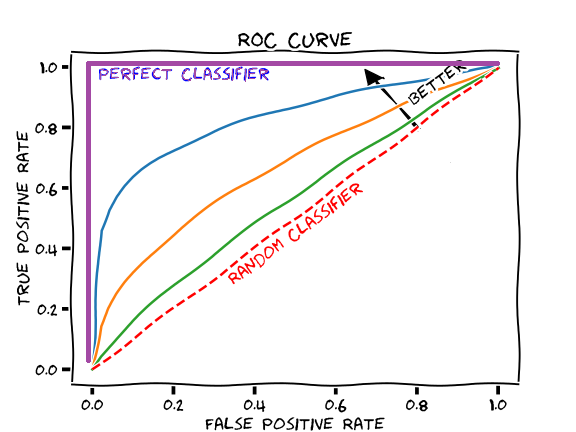
\includegraphics[width=0.6\textwidth]{imgs/roccurve.png}
\caption{ Figura esquemática donde ser observa como varían las curvas ROC de los modelos comparándolas con los casos extremos: el modelo de predicción aleatoria (peor modelo para la clasificación binaria) y el modelo ideal que siempre acierta. Créditos: The Machine Learners \url{www.themachinelearners.com/curva-roc-vs-prec-recall} }
\label{fig:roccurve}
\end{figure}

\begin{figure}[h!]
\centering
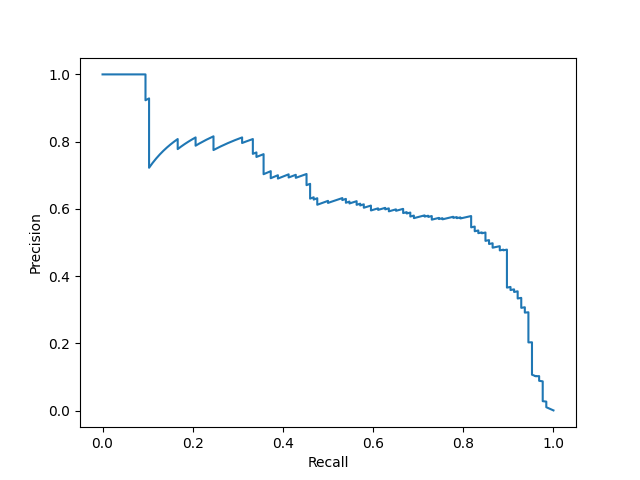
\includegraphics[width=0.6\textwidth]{imgs/precisionrecall.png}
\caption{Ejemplo de una curva de \textit{precision-recall}. Cada punto de la curva corresponde
a la \textit{precision} y el \textit{recall} obtenidos para un cierto valor de umbral de clasificación $t$.}
\label{fig:precisionrecall}
\end{figure}

La elección de métricas adecuadas es todavía más compleja en \textbf{problemas desbalanceados}, es decir, en problemas donde una de las dos clases es mucho más probable que la otra. Por ejemplo, en diagnóstico médico o detección de fraude, a menudo existen en el conjunto de datos un número pequeño de ejemplos clasificados como positivos. Esto puede acarrear que un modelo que se entrene para maximizar la \textit{tasa de aciertos} degenere en predecir siempre la clase más abundante (la negativa en los casos mencionados). No obstante, el \textit{miss rate} es crítico en los ejemplos nombrados: ¡significará fraude no detectado o patologías existentes no diagnosticadas!. \\

Existen técnicas para corregir manualmente el \textit{imbalance} de los datos como eliminar aleatoriamente parte de la clase mayoritaria (\textit{\textbf{undersampling}}) \cite{undersampling} o repetir instancias de clase minoritaria (\textit{\textbf{oversampling}}) \cite{oversampling} y técncias para que el clasificador pondere más una clase que otra \cite{desbalanceado}. 
Es de suma importancia tener en cosnideración que utilizar dichos métodos \textit{en la evaluación del modelo} muchas veces constituye un \textbf{error metodológico grave}: no se puede modificar el conjunto de datos de evaluación, ya que el mismo deberá poseer la misma distribución del hipotético conjunto de datos futuro sobre el que se aplicará el modelo (o sea, los datos que aparecerán en la aplicación final). Por ende deberán también poseer el mismo grado de \textit{imbalance}. Es por eso que las mencionadas técnicas suelen aplicarse sólo durante la fase de entrenamiento.

En éstos casos donde los datos son desbalanceados \textit{por naturaleza} lo que debemos adaptar es la estrategia de evaluación eligiendo métricas robustas al desbalance. Analizar \textit{precision} y \textit{recall} suele ser una buena opción ya que evaluaremos detectar una cierta proporción de la clase positiva pese a que sea pequeña (\textit{recall}) y tener cierta confianza en que las predicciones positivas son correctas (\textit{precision}). Para conjugar estas dos métricas y obtener una medida de perforcmance numérica es común calcular el área debajo de la curva \textit{Precision-Recall}, denominada \textbf{R-AUPRC}. Esta fórmula considera los valores de \textit{precision} y \textit{recall} para todos los valores de umbrales posibles. 

En la práctica generalmente se considera al umbral como parte del modelo final ya que son las predicciones las que se utilizarán para tomar decisiones. Una estrategia que tiene en cuenta ambas métricas a la hora de elegir el umbral  es pensar un umbral de \textit{recall} o \textit{precision} aceptado y maximizar la otra variable. 

En el caso de nuestros errores en telegramas electorales, una alerta de \textit{no coincidencia} (clase positiva) previene que se soliciten retransmisiones por telegramas mal confeccionados desde el centro de cómputo, lo cuál genera trabajo humano innecesario. Como estaremos satisfechos en reducir en $\times 5$ las retransmisiones, nos contentaremos con un \textit{recall} del $0.8$. A su vez, si el ratio de falsas alertas es alto, el usuario desestimará las alarmas, por lo que queremos que la \textit{precision} sea de al menos $0.95$ (de modo que a lo sumo $1$ de cada $20$ alarmas sean \textit{falsas alarmas}).

Puede ser interesante disponer de una forma de comparar dos modelos de predicción (habiendo fijado el umbral para cada uno). Para ello se suele combinar \textit{recall} y \textit{precision} en una única métrica utilizando el $\boldsymbol{F}$\textbf{\textit{-score}} (o $\boldsymbol{F}$\textbf{\textit{-measure}}), que es la media armónica de ambas:

\begin{equation*}
    F\text{-}score = \frac{2}{recall^{-1} + precision^{-1}} = 2 \frac{precision . recall}{precision + recall}
\end{equation*}

A veces los conjuntos de datos son generados y poseen desbalance. Ésto es algo que ocurre en los problemas de similitud que se discutirán más adelante en la tesina: generalmente poseemos varios ejemplos que pertenecen a diferentes clases (firmas de un mismo autor, caras de una persona, etc) y construimos nuestros conjuntos formando pares que constituyan \textit{coincidencias} y \textit{no coincidencias}. De este modo podemos correr el riesgo de generar conjuntos desbalanceados (por ejemplo si se toman todos los pares de elementos). En \cite{tesis-parodi} se nombra el problema de desbalanceo en los conjuntos de datos (generados como parte del mismo trabajo) como limitante para obtener mejores métricas de error sobre la clase no predominante (sección 3.9 sobre trabajos futuros). Un muestreo incorrectamente imbalanceado en la evaluación (o sea que no sigue la distribución real de los datos a los cuáles el modelo pretende generalizar) puede constituir un error metodológico grave.

\subsection{Importancia de la Metodología de Evaluación}

La metodología de evaluación es la que define como evaluar una solución al problema. En Aprendizaje Automatizado se compone fundamentalmente de la confección del conjunto de test y de la elección de la medida de performance.

No es poco frecuente encontrar trabajos con errores de conjuntos de test mal confeccionados (por ejemplo con correlaciones no generalizables al conjunto total de datos), con errores en la elección de métricas (como usar métricas tales como tasa de aciertos para problemas desbalanceados), o incluso sin conjunto de test (sólo reportan datos de validación). Éstos errores invalidan totalmente los resultados del trabajo.

La solución a un problema y la evaluación al mismo tienen intereses contrapuestos: uno puede llegar a resultados sorprendentes -pero inválidos- con una solución si se la evalúa erróneamente.  Es por ello que para garantizar que estamos haciendo un buen trabajo lo mejor es que el diseño de la metodología de evaluación del problema y las soluciones, sean responsabilidades y trabajos distintos e independientes.

Esto último sucede en el ámbito académico donde hay publicaciones que \textit{presentan} un conjunto de datos con ciertas métricas (y muchas veces un \textit{baseline}). Y luego existe un gran número de trabajos sucesivos que presentan soluciones y resultados sobre dicho problema.

También sucede en competencias de modelos donde el quién diseña el problema (incluyendo los conjuntos de datos y la manera de evaluar) y quién propone las soluciones son diferentes personas: los jueces y participantes. En las mismas, además, el puntaje sobre el conjunto de test suele ser oculto hasta terminada la competencia, evitando que se use la información de \textit{feedback} para ajustar hiperparámetros. Esto presta una mayor garantía de confianza. 

Cuando analizamos un trabajo que presenta una solución para un problema que él mismo define, hay que someterlo a un estricto escrutiño de que la metodología de evaluación sea correcta y haya sido correctamente implementada. \\

La metodología de evaluación es crítica en la práctica a la hora de desplegar soluciones que se basen en aprendizaje automático, incluso si se decide no desarrollar soluciones propias sino adquirirlas de terceros. Por ejemplo en organizaciones que van a subcontratar el proceso de desarrollo de modelos de Aprendizaje Automático, un conjunto de test correctamente construído y oculto al contratista (y preferentemente con un \textit{baseline} conocido) da la pauta de qué tan bueno es el trabajo que se estará adquiriendo.

\subsection{Reducción de la dimensionalidad}

En ocasiones resulta útil reducir la dimensionalidad de los datos para, por ejemplo, poder analizarlos visualmente utilizando 2 o 3 dimensiones que sean graficables. Un método muy utilizado es el de PCA que elije las direcciones linealmente decorrelacionadas de mayor variabilidad de los datos. 

El análisis de componentes principales (\textbf{PCA} por su nombre en inglés \textit{\textbf{Principal Component Analysis}}) es un método popular de extracción de atributos no supervisado \cite{pca}.

Podemos interpretar intuitivamente las componentes principales como las direcciones donde hay mayor variabilidad de los datos. Una vez encontradas dichas direcciones, por orden de importancia según mayor variabilidad de los datos, se puede proyectar los ejemplos, mediante un cambio de coordenadas, y quedarnos con las proyecciones respectivas a las $k$ direcciones más importantes, y así reducir la cantidad $p$ de atributos ($k < p$).\\

\begin{figure}[h!]
\centering
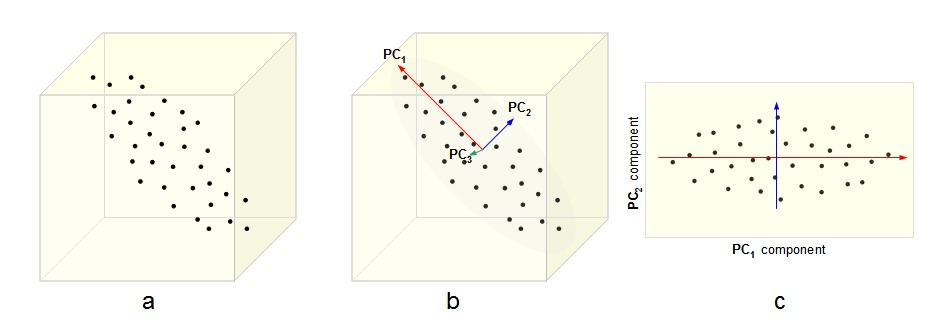
\includegraphics[width=0.8\textwidth]{imgs/pca_1.png}
\caption{ En (a) se muestra un conjunto de datos en tres dimensiones. En (b) se identifican las tres componentes principales (direcciones linealmente decorrelacionadas con mayor variabilidad de datos). En (c) se alinean los datos con las dos direcciones de mayor variabilidad (cambio de base), y se elimina la componente con menor variabilidad. Como consecuencia, la dimensionalidad de los datos se redujo en 1 y pueden ser graficados en el plano. Fuente: \url{cnx.org}  }
\label{fig:pca}
\end{figure}

PCA se calcula en cada paso buscando el versor cuya dirección sea ortogonal a las direcciones de los versores ya calculados, y que maximice la varianza de las proyecciones de los datos sobre dicha dirección. Por construcción, el conjunto de versores generados constituye una base ortonormal.

Luego de calculadas $k$ componentes principales se pueden proyectar los datos sobre dichas direcciones (cambio de base), ignorándose el resto de las componentes. La dimensionalidad se reduce a $k$, capturando -a veces también se dirá ``explicando''- la mayor variabilidad de datos que es posible capturar -o ``explicar''- con cambios de base.\\

También existen métodos de reducción de dimensionalidad que aplican transformaciones no lineales y a veces (dependiendo el conjunto de datos) pueden arrojar mejores resultados. Aún así PCA suele ser suficiente y es adoptado por su sencillez.
